% ****** Start of file apssamp.tex ******
%
%   This file is part of the APS files in the REVTeX 4.1 distribution.
%   Version 4.1r of REVTeX, August 2010
%
%   Copyright (c) 2009, 2010 The American Physical Society.
%
%   See the REVTeX 4 README file for restrictions and more information.
%
% TeX'ing this file requires that you have AMS-LaTeX 2.0 installed
% as well as the rest of the prerequisites for REVTeX 4.1
%
% See the REVTeX 4 README file
% It also requires running BibTeX. The commands are as follows:
%
%  1)  latex apssamp.tex
%  2)  bibtex apssamp
%  3)  latex apssamp.tex
%  4)  latex apssamp.tex

%Set document type
\documentclass[
  reprint,
  amsmath,amssymb,
  aps
]{revtex4-1}


%Import packages similar to importing libraries in python.
\usepackage{float}
\usepackage{physics}

\usepackage{graphicx} %Include figure files
\graphicspath{ {figures/} } % Figure file location
\usepackage{subcaption}

\usepackage{dcolumn}% Align table columns on decimal point
\usepackage{bm}% bold math

\usepackage{bookmark}

%Import this last. Allows clickable figures, equations, and links.
\usepackage{hyperref} % add hypertext capabilities
\hypersetup{
    colorlinks = true,
    linkcolor = black,
    filecolor = magenta,      
    urlcolor = cyan,
    citecolor = blue,
    }




%Latex does \begin{...} and \end{...}
\begin{document}

\title{A Quantum Mechanical Analysis of Gate Tunneling Current in MOSFETs}% Force line breaks with \\



\author{Lawrence Liu}
\affiliation{Department of Electrical and Computer Engineering, University of California\textbf{--}Los Angeles, Los Angeles, California 90095, USA}

%\date{\today}% It is always \today, today,
             %  but any date may be explicitly specified

\begin{abstract}
    This paper provides a brief overview of the operation of MOSFETs and their applications in CMOS logic gates. The 
    equations of the approximate operation characteristics of MOSFETs are presented, and then they are analyzed to 
    show how scaling the MOSFET oxide thickness affects the operation of the MOSFET. We then develop a model for the 
    tunneling current through the oxide layer of a MOSFET through Bardeen Tunneling Theory, which we used to show that the tunneling 
    current scales exponentially with decreasing oxide thickness. We then analyze the effects of tunneling current on the 
    operation of a MOSFET, and discuss ways to avoid the effects of tunneling current.
\end{abstract}

%bookmarksetup creates bookmarks at root level.
%Otherwise the title is one collapsible bookmark
\maketitle
\bookmarksetup{startatroot}

%Table of contents command
%\tableofcontents

\section{\label{sec:level1}Introduction}
Metal Oxide Semiconductor Field Effect Transistors (MOSFETs) are the most common type of transistor used in modern electronics, and 
at the heart of modern microprocessors. Let us start 
by briefly discussing the basic operation of a MOSFETs and a common application of MOSFETs in Complemetary Metal Oxide Semiconductor (CMOS) logic gates.
\subsection{\label{sec:level2}Basic MOSFET Structure}
The MOSFET is based around a Metal Oxide Semiconductor (MOS) capacitor. Historically this 
was a gate made out of a metal plate on top of a semiconductor substrate, which was separated by an insulating layer of oxide, however modern 
MOSFETs use a polysilicon gate instead of a metal gate.\\\\
Now to make a MOSFET we add a source and drain silicon regions to the silicon substrate. The source and drain regions are doped with impurities to
be the opposite type to that of the base silicon substrate. For example, if the base silicon substrate is p-type, then the source and drain regions
are n-type, and vice versa. We call the MOSFET with n-type source and drain regions an nMOSFET, and the MOSFET with p-type source and drain regions. We have 
drawn both an nMOSFET and a pMOSFET in Figure (\ref{fig:nmosfet} and \ref{fig:pmosfet}) along with their respective circuit symbols.\\\\
\begin{figure}[H]
    \centering
    % \begin{subfigure}[b]{0.3\textwidth}
        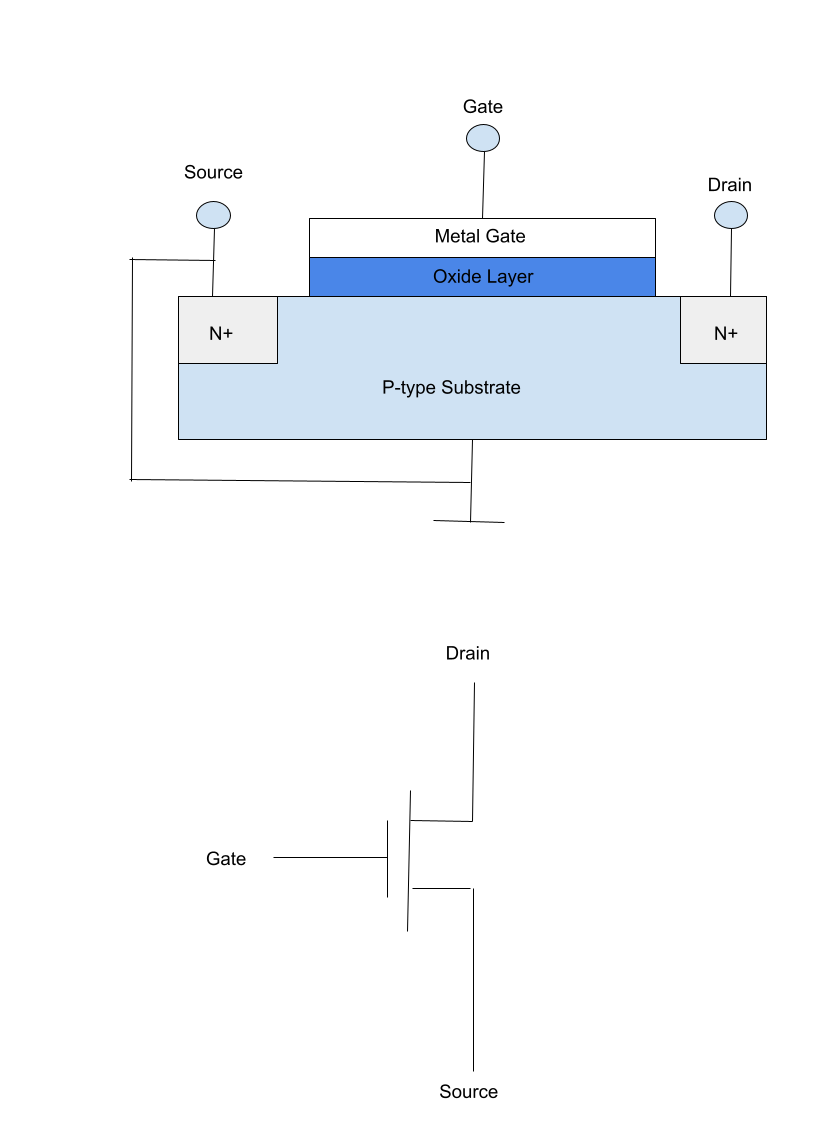
\includegraphics[width=0.45\textwidth]{nmosfet.png}
        % \caption{nMOSFET}
        % \label{fig:nmosfet}
    % \end{subfigure}
    % \begin{subfigure}[b]{0.3\textwidth}
    %     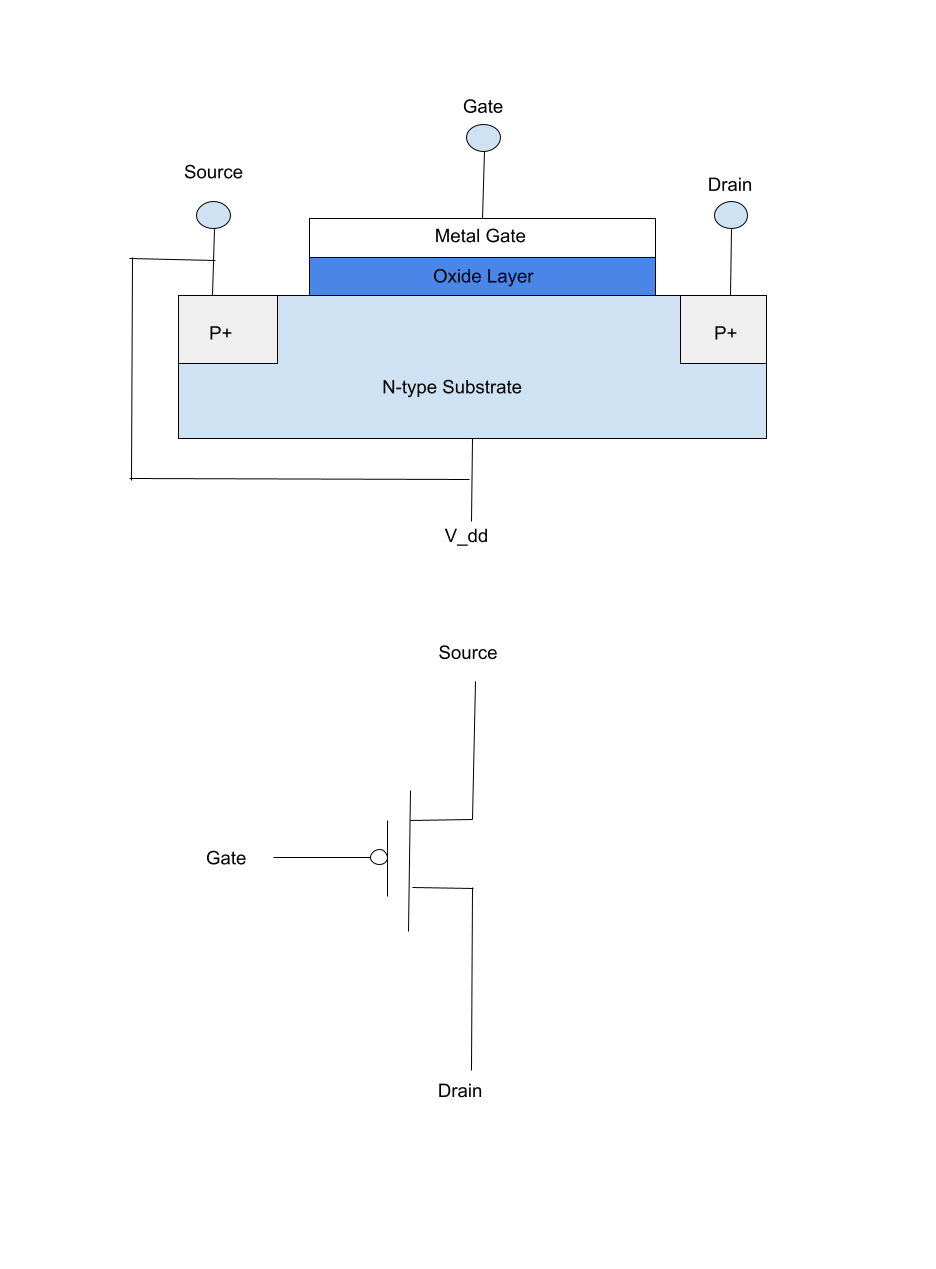
\includegraphics[width=\linewidth]{pmosfet.png}
    %     \caption{pMOSFET}
    %     \label{fig:pmosfet}
    % \end{subfigure}
    \caption{A diagram of an nMOSFET and its circuit symbol.}
    \label{fig:nmosfet}
\end{figure}
\begin{figure}[H]
    \centering
    % \begin{subfigure}[b]{0.3\textwidth}
        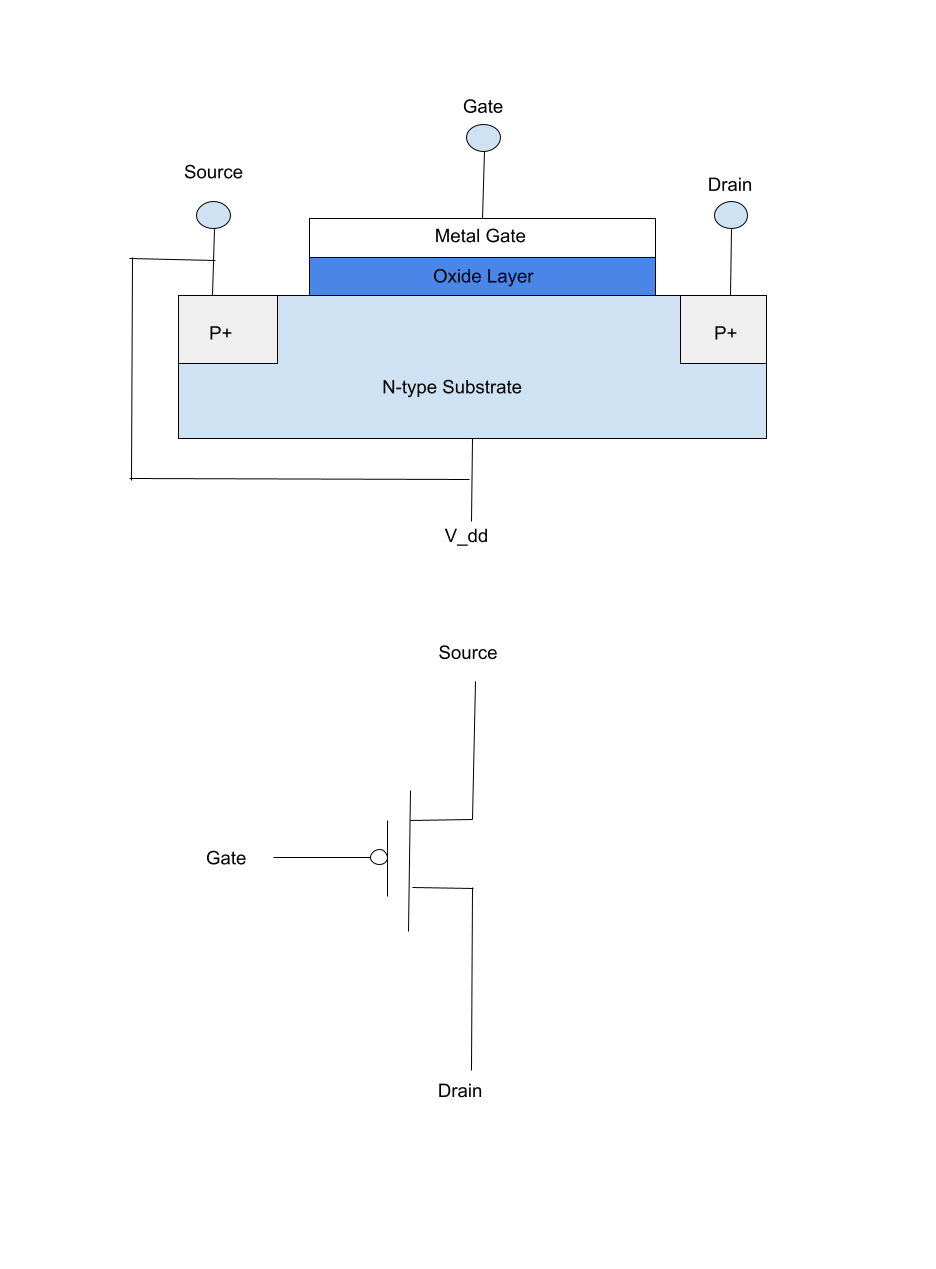
\includegraphics[width=0.45\textwidth]{pmosfet.png}
        % \caption{nMOSFET}
        % \label{fig:nmosfet}
    % \end{subfigure}
    % \begin{subfigure}[b]{0.3\textwidth}
    %     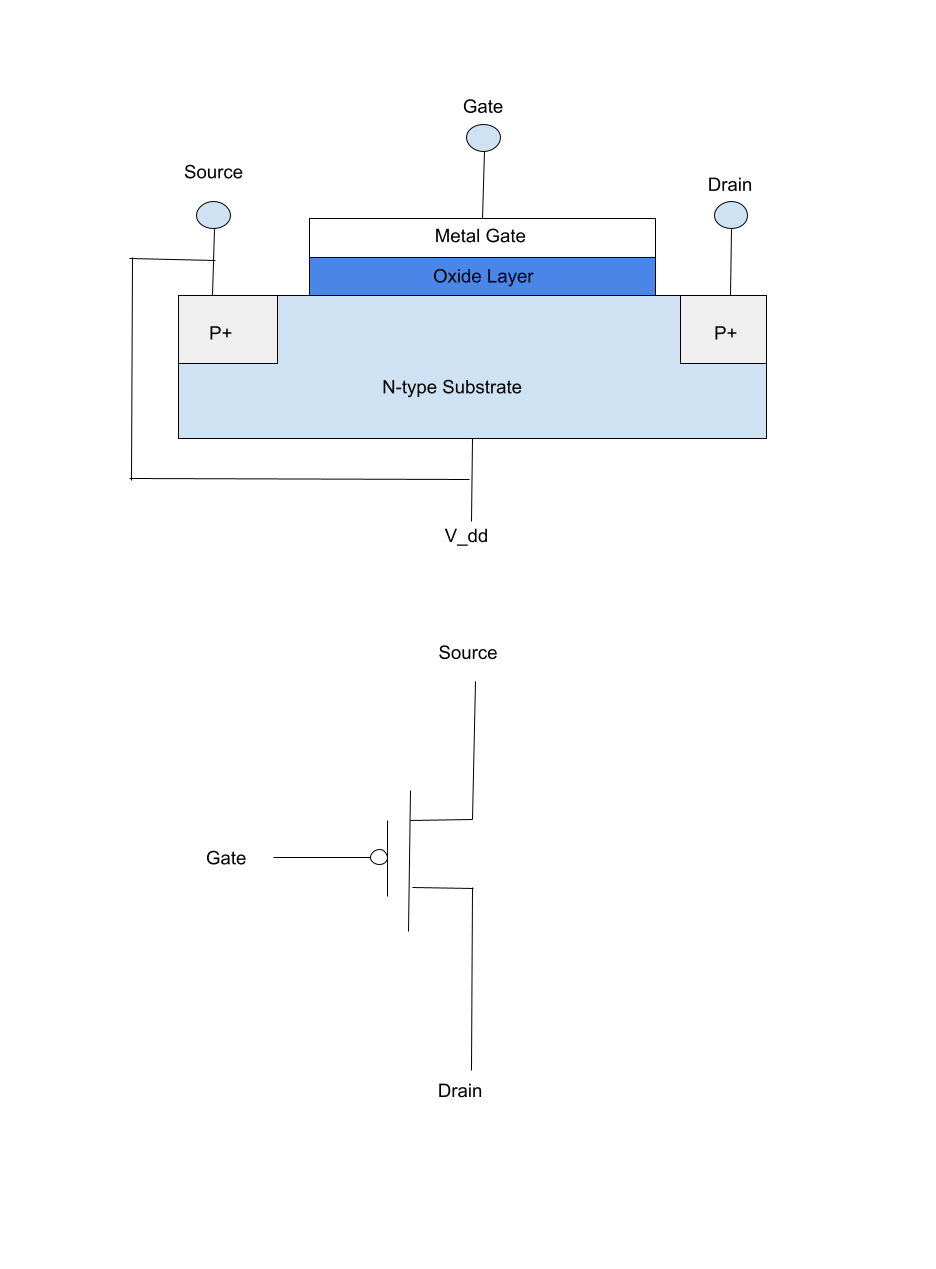
\includegraphics[width=\linewidth]{pmosfet.png}
    %     \caption{pMOSFET}
    %     \label{fig:pmosfet}
    % \end{subfigure}
    \caption{A diagram of an pMOSFET and its circuit symbol.}
    \label{fig:pmosfet}
\end{figure}
Let us define $V_{ds}$ as the voltage between the drain and source, and $V_{gs}$ as the voltage between the gate and source.
\subsection{\label{sec:level2}MOSFET Operation}
Now let us consider a the operation of a nMOSFET in a qualitative sense. If we apply a positive voltage to the gate, then 
the holes in the p-type substrate will be pushed away from the gate, or more accurately, the minority electrons will be drawn 
to the gate. If enough are drawn to the gate, then an inversion layer of n-type Silicon will form at the surface of the substrate since 
enough electrons will be present to become the majority carrier. This inversion layer will form a conductive channel between the source and drain, 
allowing current to flow between the source and drain. Therefore in a very rough sense, we can see that a MOSFET acts 
as a voltage controlled switch.\\\\
In a more rigorous sense, what happens is that the gate voltage "bends" the energy bands in the p-type substrate lower. 
Once these bands bend to the degree that near the surface of the substrate, the conduction band is closer to the 
Fermi level than the valence band, then the inversion layer will form. This threshold is given by \cite{ChenmingHu5}
\begin{equation}
    V_{T} = V_{FB} + 2\phi_{B} + \frac{Q_{SS}}{C_{OX}}
    \label{eq:threshold_nMOSFET}
\end{equation}
Where $V_{FB}$ is the flatband voltage, ie the difference in the work functions of the gate and the substrate, $\phi_{B}$ is the 
difference between the Fermi level and the intrinsic Fermi level divided by the electron charge, $Q_{SS}=\sqrt{2\epsilon_{s}qN_{a}(2\phi_{B})}$ where 
$N_a$ is the doping concentration of the substrate, and $C_{OX}$ is the capacitance of the oxide layer.\\\\
We can see that the opposite happens for a pMOSFET. If we apply a negative voltage to the gate, then since the electrons are pushed 
away and the holes are drawn to the gate, then an inversion layer of p-type Silicon will form at the surface of the substrate. Or 
from a bands perspective, the bands will be "bended" upwards to the degree that the valence band is closer to the Fermi level than the
conduction band. We have that this threshold is given by \cite{ChenmingHu5}
\begin{equation}
    V_{T} = V_{FB} - 2\phi_{B} - \frac{2\epsilon_{s}qN_{d}(2\phi_{B})}{C_{OX}}
    \label{eq:threshold_pMOSFET}
\end{equation}
Where $N_d$ is the doping concentration of the substrate.\\\\
Thus when we a apply a voltage greater or less than the threshold voltage for the nMOSFET and pMOSFET respectively, then the inversion layer will form. We 
can view this layer as a effectively a resistor between the source and drain. However as we increase the current across the 
drain and the source $V_{DS}$, we will start to experience "pinch off" where the inversion layer will start to narrow. Once the 
voltage is high enough, the inversion layer will pinch off completely, and no longer connect the source and drain. This is 
depicted in Figure \ref{fig:mosfet pinch off}. This will cause the MOSFET to no longer act as a voltage controlled 
resistor between the source and drain, and instead act as a voltage controlled current source. We call this 
operation region the "saturation" region as opposed the "Ohmic" region where the MOSFET acts as a voltage controlled resistor.\\\\
\begin{figure}
    \centering
    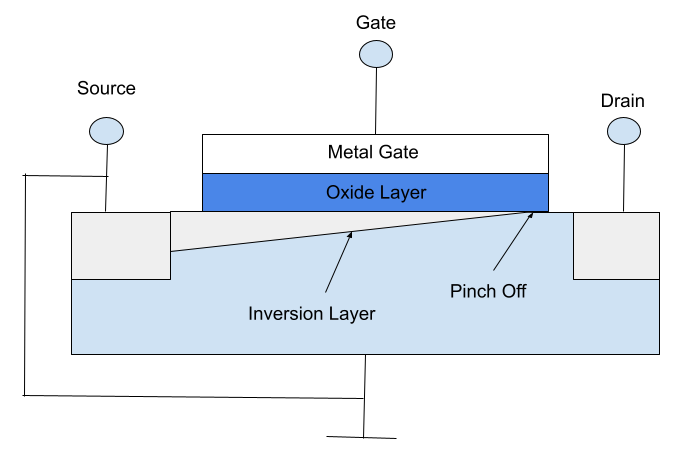
\includegraphics[width=0.9\linewidth]{mosfet_pinch_off.png}
    \caption{Pinch off in a MOSFET.}
    \label{fig:mosfet pinch off}
\end{figure}
The threshold for $V_{DS}$ at which the MOSFET enters the saturation region can be approximated by \cite{ChenmingHu6}
\begin{equation}
    V_{DS,sat} = V_{GS} - V_{T}
\end{equation}
The current in the saturation region therefore can be approximated by\cite{ChenmingHu6}
\begin{equation}
    I_{D,sat} = \frac{1}{2}C_{OX}\frac{W}{L}(V_{GS}-V_{T})^{2}
    \label{eq:mosfet saturation current}
\end{equation}
Where $W$ is the width of the MOSFET and $L$ is the length of the MOSFET.
\subsection{\label{sec:level2}Examples of MOSFET based circuits}
Now with this understanding of the operation of a MOSFET, we can now look at some examples of MOSFET based circuits.
\subsubsection{\label{sec:level3}CMOS Inverter}
By connecting a pMOSFET and a nMOSFET in series, we can create a CMOS inverter. This is depicted in Figure \ref{fig:cmos inverter}.\\\\
\begin{figure}[H]
    \centering
    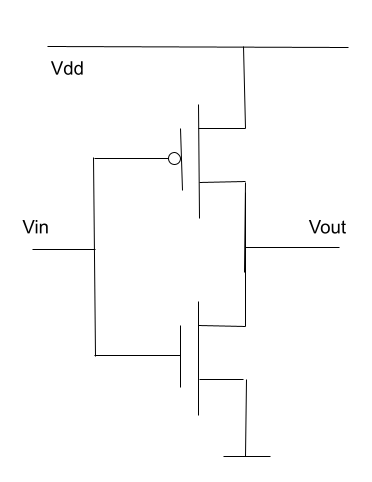
\includegraphics[width=0.75\linewidth]{cmos_inverter.png}
    \caption{CMOS inverter.}
    \label{fig:cmos inverter}
\end{figure}
To understand this circuit let us consider two cases when the input is "low" and when the input is "high". Let us assume that 
we have biased the circuit such that the threshold voltage of the nMOSFET is equal to the threshold voltage of the pMOSFET. Then in the 
case where the input is low, then the nMOSFET will be effectively an open circuit, and the pMOSFET will be effectively a closed circuit. Therefore the output will be high. 
Conversely, if the input is high, then the nMOSFET will be effectively a closed circuit, and the pMOSFET will be effectively an open circuit. 
Therefore the output will be low. Thus we can see that this circuit acts as an inverter. Likewise we can create more 
complex cirucits to implement logic gates such as a NAND or NOR gate using CMOS, which are discussed in Appendix A.
\subsection{\label{sec:leve2}Speed}
We should note that a MOSFET is not an instantaneous switch, we can create an basic approximation by 
considering the MOSFET as a RC circuit. The capacitance comes from various wires connecting the MOSFET, and the capacitance that is formed in the 
PN junction between the source and drain and the substrate. We can add this capacitance to the MOSFET model as depicted in figure (\ref{fig:cmos_train}) for a 
CMOS inverter train.\\\\
\begin{figure}[H]
    \centering
    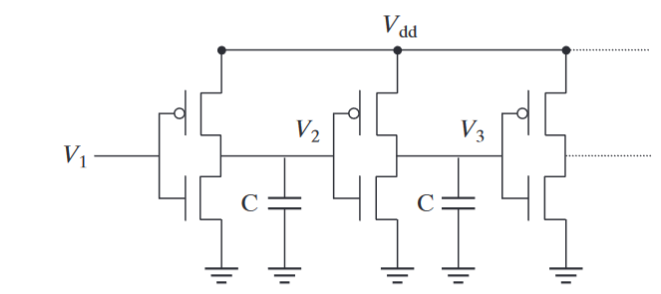
\includegraphics[width=0.75\linewidth]{cmos_inverter_train.png}
    \caption{CMOS inverter train, figure from \textit{Modern Semiconductor Devices for Integrated Circuits} by Chenming C. Hu. \cite{ChenmingHu6}}
    \label{fig:cmos_train}
\end{figure}
We can approximate the switching resistance of the MOSFET as $R\approx \frac{V_{dd}}{2I_{on}}$, Thus we have that 
the switching delay is proportional to the RC time constant of the MOSFET. We have that:
\begin{equation}
  \tau \propto \frac{C}{I_{on}}V_{DD}
\end{equation}
\section{\label{sec:level1}MOSFET Sizing}
Now armed with the knowledge of how MOSFETs work, let us examine how the size of a MOSFET can affect its performance, and why 
it is beneficial to have a smaller MOSFET. The most intuitive reason is that a smaller MOSFET will alow us to fit more MOSFETs
on a single chip, which allows for more digital circuits to be implemented on 
one chip, and thus driving down the cost per circuit.\\\\
Furthermore, by modifying other parameters of the MOSFET size, we
can also increase the speed and power efficiency of the MOSFET. 
Let us consider the capacitance of the Oxide layer of a MOSFET. We have that if the Oxide has a thickness of $t_{ox}$, 
an area of $A$, and a dielectric constant of $\epsilon_{ox}$, then the capacitance of the oxide layer is given by
\begin{equation}
  C_{ox} = \frac{\epsilon_{ox}A}{t_{ox}}
\end{equation}
Now if we consider a MOSFET with a thinner oxide layer $\alpha t_{ox}$ we 
have that the capacitance of the oxide layer is given by
\begin{equation}
  C_{ox} = \frac{\epsilon_{ox}A}{\alpha t_{ox}}
\end{equation}
Therefore we can see that the capacitance of the oxide layer is inversely proportional to the thickness of the oxide layer. Now if we return to 
equations (\ref{eq:threshold_nMOSFET}) and (\ref{eq:threshold_pMOSFET}), we can see that the threshold voltage is varies inversely proportional to the capacitance of the oxide layer. 
Thus a thinner oxide layer will have a lower threshold voltage. This is important because a lower threshold voltage means that the MOSFET will require less voltage, and therefore 
at a same current, will dissipate less power.\cite{ChenmingHu6}\\\\
This will also affect the speed of the MOSFET by increasing the on current. We have that the on current given by 
equation (\ref{eq:mosfet saturation current}) is proportional to $(V_{GS}-V_{T})^{2}$. Therefore a lower threshold voltage will result in 
a higher on current. Now if we recall that the switch time of a MOSFET is proportional to $\frac{1}{I_{on}}$. Therefore 
a smaller threshold voltage will result in a faster switch time, or alternatively a lower power dissipation for the 
same switching time.\cite{ChenmingHu6}\\\\
\subsection{\label{sec:level2}Issues with MOSFET Scaling}
Then what would stop us from making our MOSFETs smaller and smaller? Well, there will be several issues that will 
arise as we make our MOSFETs smaller. Of course the most obvious issue is that it will be harder to manufacture smaller MOSFETs. Furthermore, 
as we make our MOSFETs smaller, the behaviour of the MOSFET will be less dependent on the Classical Physics that the pervious 
equations were derived from. As an example, we will examine how scaling down the 
MOS capacitor will cause Quantum Tunneling to become a significant factor in the behaviour of the MOSFET. We will 
then examine how this will affect the behaviour of the MOSFET and how we can mitigate this effect.\\\\
\section{\label{sec:level1}Bardeen Tunneling Theory}
Let us start by briefly summarizing Bardeen Tunneling Theory. Let us consider a quantum mechanical system as depicted in 
Figure \ref{fig:bardeen tunneling} consisting of two potential wells separated by a barrier:\\\\
\begin{figure}[H]
    \centering
    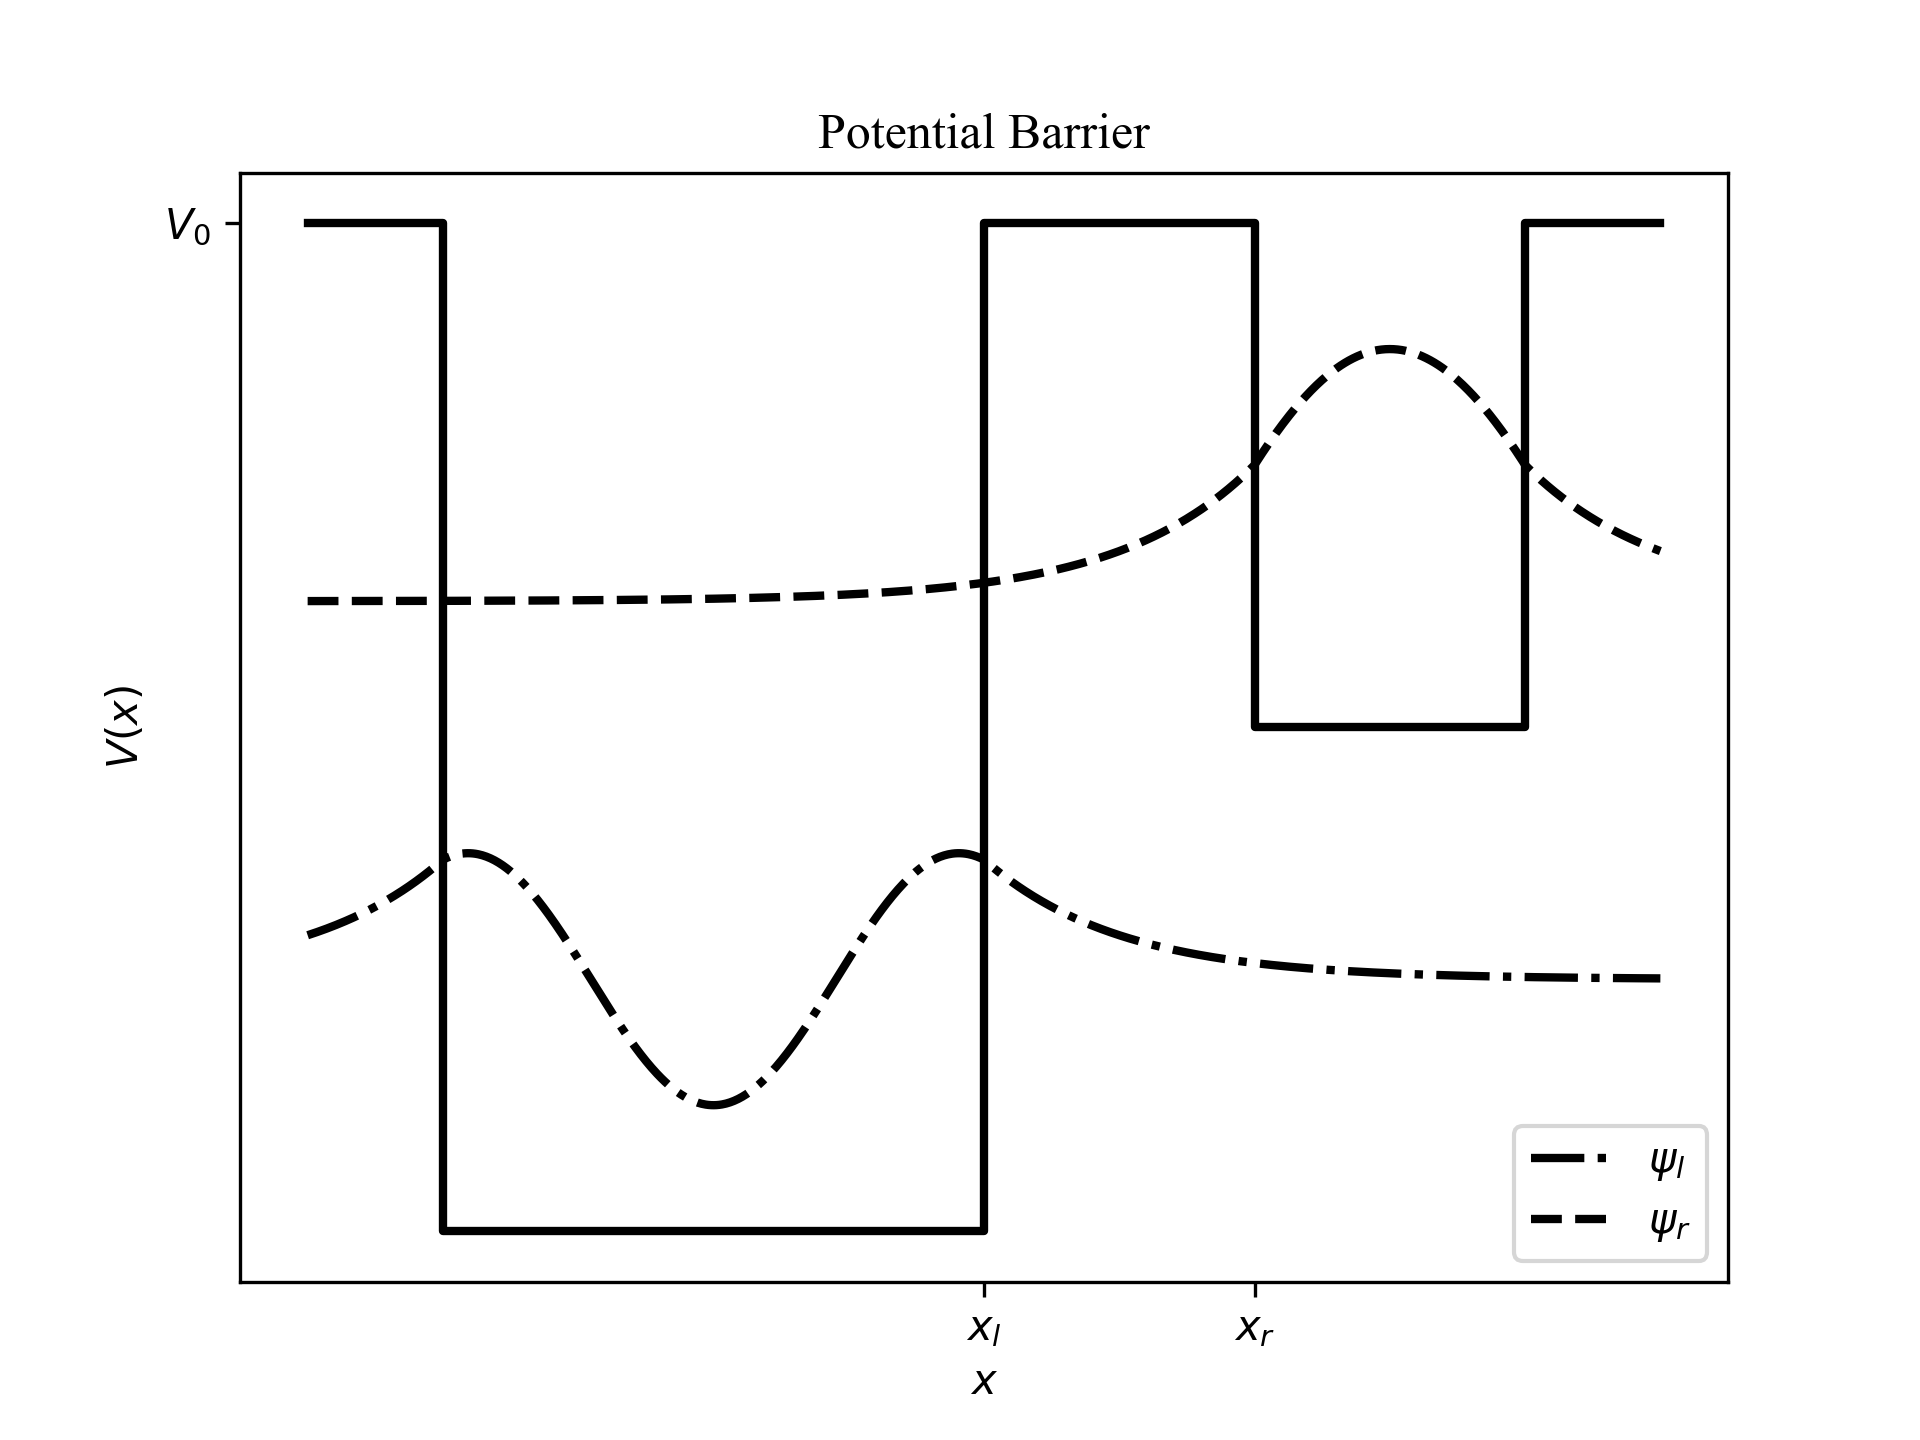
\includegraphics[width=0.9\linewidth]{bardeen_tunneling.png}
    \caption{Potential wells and wavefunctions.}
    \label{fig:bardeen tunneling}
\end{figure}
As we depicted, let us assume that both of these potential wells are symmetric around their own origins, and thus 
the potential outside the well is the same, which we defined in figure (\ref{fig: bardeen tunneling}) to be $V_0$. 
Then we have that the potential is given by
\begin{equation}
    V(x) = \begin{cases}
        V_l(x) & x < x_1\\
        V_r(x) & x \geq x_1
    \end{cases}
\end{equation}
Where $V_l(x)$ is the potential function for the left well, and $V_r(x)$ is the potential function for the right well, and 
$x_1$ is some arbitrary point $x_l<x_1<x_r$. We can see that we can express this as: 
\begin{equation}
    V(x) = V_l(x) - \Theta(x-x_1)(V_0-V_r(x))
\end{equation}
Where $\Theta(x)$ is the Heaviside step function. 
Therefore we can see that we can write the hamiltonian for this system as:
\begin{equation}
    H = \frac{p^2}{2m} + V_l(x) - \Theta(x-x_1)(V_0-V_r(x))
\end{equation}
We can see that if we define $H_l$ as the hamiltonian of a system consisting solely of the left well, and $H' = 
\theta(x-x_1)(V_0-V_r(x))$, then we can write the hamiltonian as:
\begin{equation}
    H = H_l + H'
\end{equation}
Therefore we can see the that the tunneling rate can be modeled by with Fermi's Golden Rule, with $H'$ as the perturbation that 
turns on at $t=0$. If we 
make the key assumption that the energy of the left well is approximately equal to the energy of the right well, ie 
$E_l \approx E_r =E$. We have that the transition rate is given by:
\begin{equation}
    \Gamma_{l\rightarrow r} = \frac{2\pi}{\hbar}\abs{\bra{r}H'\ket{l}}^2\rho(E)
\end{equation}
We have that the matrix element is given by:
\begin{equation}
    \bra{r}H'\ket{l} = \int_{-\infty}^{\infty}\psi_r^*(x)H'\psi_l(x)dx
\end{equation}
After doing some simplifications derived in Appendix B, and with the assumption that $E_l \approx E_r =E$ we have that the matrix element is given by:
\begin{equation}
    \bra{r}H'\ket{l} = \frac{\hbar^2}{2m}\left(
        \psi_r^*\frac{d}{dx}\psi_l - \psi_l\frac{d}{dx}\psi_r^*
    \right)\Bigg|_{x=x_1}
\end{equation}
Which is the central result of Bardeen Tunneling Theory. \cite{BardeenTunneling}.

\subsection{\label{sec:level2}Application to MOSFETs}
Now let us use it to try to approximate the gate source tunneling current 
of a MOSFET. We model the potentials and for a electron in the 
gate and substrate as two finite square wells, as depicted in figure (\ref{fig: bardeen tunneling}), and with the 
raised potential barrier as a crude model of the oxide layer. Recall that 
wavefunction for a particle in a finite square well of length  $L$ centered at $x=0$ is given by:
\begin{equation}
    \psi(x) = \begin{cases}
        A\frac{e^{-K\frac{L}{2}}}{\cos(K\frac{L}{2})}\cos(Kx) & |x|<\frac{L}{2}\\
        Ae^{-k|x|} & |x|>\frac{L}{2}
    \end{cases}
\end{equation}
Where $K = \frac{1}{\hbar}\sqrt{2m(V-E)}$, $k=\frac{1}{\hbar}\sqrt{2mE}$, and $A$ is a normalization constant, and $V$ is the height of the 
walls of the box. Then we have that 
the matrix element is given by:
\begin{multline}
    \bra{r}H'\ket{l} = \frac{\hbar^2}{2m}\left(
        A_re^{-k_r x} \frac{d}{dx}A_le^{k_l \left(x-L_{b}-\frac{L_l+L_r}{2}\right)}\right. -\\
         \left.A_le^{k_l \left(x-L_{b}-\frac{L_l+L_r}{2}\right)}\frac{d}{dx}A_re^{-k_r x}\right)
\end{multline}
Where $L_b$ is the length of the barrier, $L_l$ is the length of the left well, and $L_r$ is the length of the right well. 
Likewise if we note that since we assumed with the Bardeen Tunneling Theory that the energy of the particle in the 
left well is approximately equal to the energy of the particle in the right well, we have that $k_l \approx k_r = k$. Thus we 
have that the matrix element is given by:
\begin{equation}
    \bra{r}H'\ket{l} = -\frac{\hbar^2}{m}A_l A_r k e^{-k\left(L_b+\frac{L_l+L_r}{2}\right)}
\end{equation}
Therefore we can see that the tunneling rate is given by:\\\\
\begin{equation}
    \Gamma_{l\rightarrow r} = \frac{2\pi}{\hbar}\frac{\hbar^4}{m^2}A_l^2 A_r^2 k^2 e^{-2k\left(L_b+\frac{L_l+L_r}{2}\right)}\rho(E)
\end{equation}
Now for our case, since the barrier is the dielectric layer, we have that $L_b = t_{ox}$. Furthermore, we have that the tunneling current is given by:\\\\
\begin{equation}
    I_{tunnel} = q\Gamma_{l\rightarrow r}
\end{equation}
Thus we can see that from this crude model of the MOSFET, we can see that the tunneling current scales exponentially with the
$-t_{ox}$. This is reflected in the actual data of the gate source tunneling current compared with the oxide thickness, as
we showed in figure (\ref{fig: gate source tunneling current}). This approach for modeling the tunneling current was based 
on the paper \textit{Theory of direct tunneling current in metal-oxide-semiconductor structures} by Clerc et al. \cite{Clerc}
\begin{figure}[H]
    \centering
    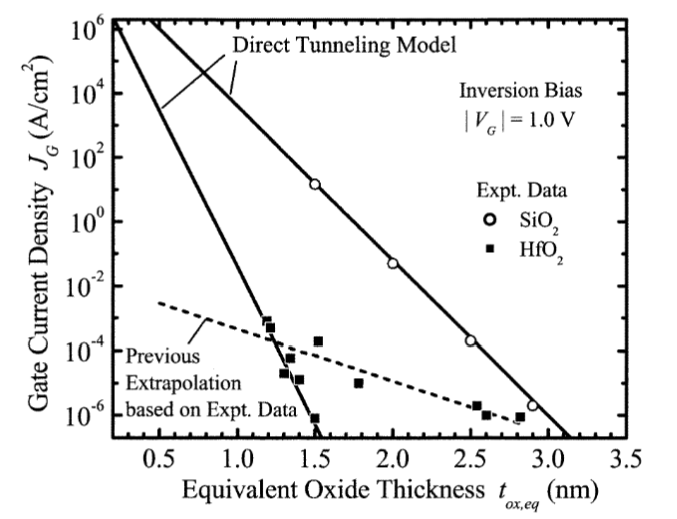
\includegraphics[width=0.75\linewidth]{Gate Current Density vs Oxide Thickness.png}
    \caption{Gate Source Tunneling Current Density vs Oxide Thickness, figure from \textit{MOSFET Gate Leakage Modeling and Selection
    Guide for Alternative Gate Dielectrics
    Based on Leakage Considerations} by Yee-Chia Yeo, Tsu-Jae King, and Chenming Hu \cite{Yeo}}
    \label{fig: gate source tunneling current}
\end{figure}

\subsection{\label{sec:level2}Consequences of Gate Source Tunneling and Mitigation Methods}
As was shown in figure (\ref{fig: gate source tunneling current}), at $1.2$nm the gate source leakage current is 
roughly $10^{3} A/cm^2$. Thus if we had a chip that consisted of MOSFETs with a total area of $1mm^2$,
 we would have a leakage current of $10A$. This would drain a 
phone battery (which has a capacity of $~3000mAh$) in $~10$ minutes. Therefore it is not suitable to continue to 
scale down the oxide thickness. Thus we want to find ways to mitigate the gate source tunneling current, while 
still keeping the benefits of the resulting higher $C_{ox}$ we discussed earlier.\\\\
A common solution to this problem is to use a high-k dielectric,\cite{ChenmingHu7} such as HfO$_2$ instead of the traditional SiO$_2$. HfO$_2$ has 
a dielectric constant that is roughly $6$ times that of SiO$_2$, thus we can see that we can get the same $C_{ox}$ with a 
6 times thicker HfO$_2$ layer. However since the tunneling current scales exponentially with the thickness of the oxide layer,
this will have a significantly smaller gate source leakage, which can also be seen in figure (\ref{fig: gate source tunneling current}).
\subsection{\label{sec:level2}Ways to Improve the Model}
While our model was able to capture the exponential dependence of the gate source tunneling current on the oxide thickness, it 
is not able to capture the magnitude of the gate source tunneling current. This is because we made a number of simplifying factors, 
most importantly we assumed the potential in the gate oxide is flat, however we are applying a voltage across the gate oxide, so the barrier 
will be trapezoidal and not rectangular as depicted in figure (\ref{fig: trapezoidal barrier}). To model these 
effects we would need to use WKB approximation, which was beyond the scope of this class and this paper, however the predictions of 
such a model is depicted as the Direct Tunneling Model line in figure (\ref{fig: gate source tunneling current}).\\\\
\begin{figure}
    \centering
    \includegraphics*[width=0.75\linewidth]{gate_potential_WKB.png}
    \caption{Trapezoidal model for the Gate potential, figure from \textit{Quantum Mechanical
    Effects on Mosfet Scaling Limit} by Lihui Wan \cite{Wan}}
    \label{fig: trapezoidal barrier}
\end{figure}
Likewise we also only considered direct tunneling, however at higher thicknesses other effects begin to dominate 
such as trap-assisted tunneling. This is show in the figure (\ref{fig: gate source tunneling current}), where we can see that 
for high thicknesses of HfO$_2$, the gate current density no longer begins to behave according the direct tunneling models.\cite{Yeo}

\section{\label{sec:level1}Conclusion}
In this paper we have discussed the physics of MOSFETs, and how they are used in modern day electronics. We then demonstrated 
why it is important to scale down size of a MOSFET, specifically the gate oxide thickness, and how that would result in 
performance imporvements. We then discussed the physics of gate source tunneling, derived the Bardeen Tunneling Theory, and a 
model for the gate source tunneling current based on the Bardeen Tunneling Theory. Finally we discussed the consequences of this 
tunneling current, and how to mitigate it.



\bibliographystyle{abbrv}%Used BibTeX style is unsrt
\bibliography{references}

%add appendix
\appendix
\section{MOSFET Logic Gates}
\subsection{NAND Gate}
Here we discuss an example of a CMOS logic gate, the NAND gate. 
The NAND gate is a universal gate, meaning that any boolean function can be constructed using only NAND gates. We have 
drawn an example of a NAND gate in figure (\ref{fig: NAND gate}).\\\\
\begin{figure}[H]
    \centering
    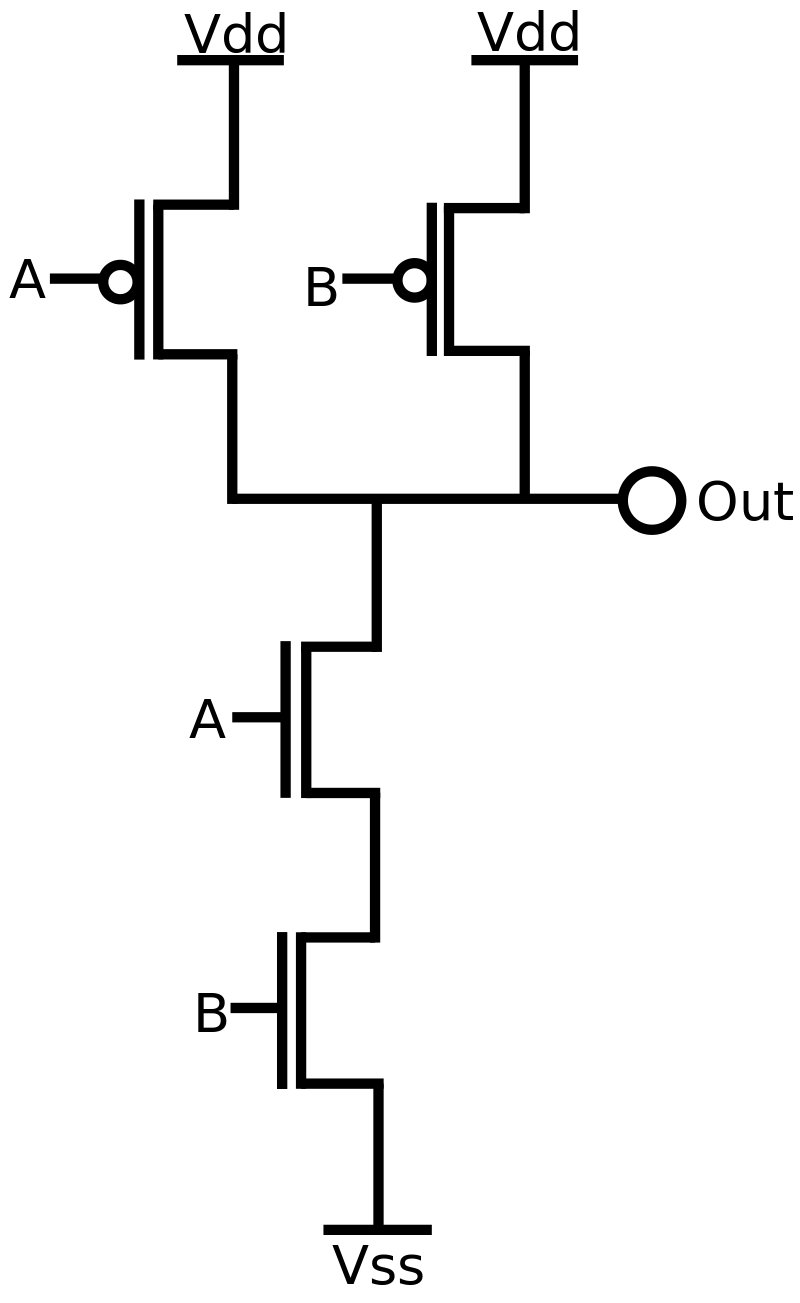
\includegraphics[width=0.75\linewidth]{cmos_nand_gate.png}
    \caption{NAND Gate, figure By JustinForce - Own work, CC BY-SA 3.0, https://commons.wikimedia.org/w/index.php?curid=2593317}
    \label{fig: NAND gate}
\end{figure}
As we can see, the NAND gate consists of two PMOS transistors in parallel with two NMOS transistors in series. Thus if both A and 
B are high, then both NMOS transistors will be on, and the PMOS transistors will be off, thus the output will be low. If either A or B 
or both are low, then at least one of the NMOS transistors will be off and at least one of the PMOS transistors will be on, thus the
output will be high.
\section{Derivation of the Bardeen Tunneling Theory}
We have that the matrix element as we established previously is 
\begin{equation}
    \bra{r}H'\ket{l} = \int_{-\infty}^{\infty}\psi_r^*(x)H'\psi_l(x)dx
\end{equation}
However since $H' = -\Theta(x-x_1)(V_0-V_r(x))$ we have that 
\begin{equation}
    \bra{r}H'\ket{l} = \int_{x_1}^{\infty}\psi_r^*(x)H'\psi_l(x)dx
\end{equation}
We also have that $H' = H_l-H$ therefore we get:
\begin{align}
    \bra{r}H'\ket{l} &= \int_{x_1}^{\infty}\psi_r^*(x)(H_l-H)\psi_l(x)dx\\
    &= \int_{x_1}^{\infty}\psi_r^*(x)(H_l+\frac{\hbar^2}{2m}\frac{d^2}{dx^2}-V_r(x))\psi_l(x)dx\\
    &= \int_{x_1}^{\infty}\psi_r^*(x)(E_l+\frac{\hbar^2}{2m}\frac{d^2}{dx^2}-V_r(x))\psi_l(x)dx
\end{align}
If we perform integration by parts we get:
\begin{align*}
    \int\psi_r^*(x)\frac{d^2}{dx^2}\psi_l(x)dx =& \psi_r^*(x)\frac{d}{dx}\psi_l(x)- \int\frac{d}{dx}\psi_r^*(x)\frac{d}{dx}\psi_l(x)dx\\
    =& \psi_r^*(x)\frac{d}{dx}\psi_l(x) - \psi_l(x)\frac{d}{dx}\psi_r^*(x)\\
    & + \int\psi_l(x)\frac{d^2}{dx^2}\psi_r^*(x)dx
\end{align*}
Therefore since $\frac{d}{dx}\psi_l\big|_{x=\infty} = \frac{d}{dx}\psi_r\big|_{x=\infty} = 0$ we get:
\begin{align*}
    \bra{r}H'\ket{l} =& \frac{\hbar^2}{2m}\left(\psi_r^*(x)\frac{d}{dx}\psi_l(x) - \psi_l(x)\frac{d}{dx}\psi_r^*(x)\right)\big|_{x=x_1}\\
            &-E_l\int_{x_1}^{\infty}\psi_r^*(x)\psi_l(x)dx+
            \int_{x_1}^{\infty}\psi_l(x)H_r\psi_r^*(x)dx\\
            =& \frac{\hbar^2}{2m}\left(\psi_r^*(x)\frac{d}{dx}\psi_l(x) - \psi_l(x)\frac{d}{dx}\psi_r^*(x)\right)\big|_{x=x_1}\\
            &+(E_r-E_l)\int_{x_1}^{\infty}\psi_r^*(x)\psi_l(x)dx
\end{align*}
Since we assume that $E_r=E_l$ we get:
\begin{equation}
    \bra{r}H'\ket{l} = \frac{\hbar^2}{2m}\left(\psi_r^*(x)\frac{d}{dx}\psi_l(x) - \psi_l(x)\frac{d}{dx}\psi_r^*(x)\right)\big|_{x=x_1}
\end{equation}
\end{document}